\documentclass[11pt]{article}
\usepackage{fullpage}
\usepackage{amsmath}
\usepackage{amsfonts}
\usepackage{setspace}
\usepackage{listings}
\usepackage{verbatim}
\usepackage{algpseudocode}
\usepackage{algorithm}
\algblockdefx[IF]{If}{EndIf}[1]{\algorithmicif\ #1}{\algorithmicend}
\algblockdefx[WHILE]{While}{EndWhile}[1]{\algorithmicwhile\ #1}{\algorithmicend}
\usepackage{galois}
\usepackage{tikz}
\usepackage{varwidth}
\usetikzlibrary{positioning}
\usetikzlibrary{arrows.meta,bending,automata}
\usepackage{pxfonts}
\usepackage[T1]{fontenc}
\lstdefinelanguage{julia}{
  basicstyle=\small\ttfamily,
  showspaces=false,
  showstringspaces=false,
  keywordstyle={\textbf},
  morekeywords={if,else,elseif,while,for,begin,end,quote,try,catch,return,local,abstract,function,stagedfunction,macro,ccall,finally,typealias,break,continue,type,global,module,using,import,export,const,let,bitstype,do,in,baremodule,importall,immutable},
  escapeinside={~}{~},
  morecomment=[l]{\#},
%  commentstyle=\textsf,
  commentstyle={},
  morestring=[b]",
}
\newcommand{\F}{\mathcal{F}}
\renewcommand{\P}{\mathcal{P}}
\newcommand{\eps}{\varepsilon}
\renewcommand{\phi}{\varphi}
\newcommand{\D}{\Diamond}
\newcommand{\uD}{\underline{\Diamond}}
\newcommand{\UD}{\overline{\Diamond}}
\renewcommand{\S}{\mathcal{S}}
\newcommand{\oS}{\overline{\mathcal{S}}}
\newcommand{\ra}{\rightarrow}
\newcommand{\lfp}{\text{lfp}}
\title{\vspace{-6ex}A modular abstract interpreter for Julia \\ MPRI internship report}
\author{Oscar Blumberg, supervised by Prof.\@ Alan Edelman, MIT}
\date{2015}
\begin{document}
\onehalfspacing
\maketitle
%\pagestyle{empty} %
\thispagestyle{empty}
\vspace{1.5ex}
\subsection*{General context}

Julia is a dynamically typed, JIT compiled, programming language implementation with an emphasis on generic programming through a powerful -- and ubiquitous -- symmetric, dynamic multiple dispatch mechanism. It achieves run-time performance untypical of other similar dynamic languages by relying heavily on static analysis and aggressive code specialization. It is meant to provide a tool for scientific computations that is both familiar and fast enough for this demanding usage. The julia compiler provides a range of meta programming and code generation techniques to the advanced user.

Efforts into optimizing dynamic languages are not new, as the common lisp tradition shows, and more recently the sizable effort into making various javascript engines high performance. Julia has the interesting advantage of having been designed from the ground up to be a good analysis target and, while being dynamic, avoids pathological behavior patterns that are very hard to infer statically.

\subsection*{Studied problem}

Most optimizations in the julia compiler are done by the LLVM library in the backend. LLVM is a widely used, production-grade compiler and generally generates excellent machine code. However, its intermediate representation operates at an abstraction level comparable to that of C.

Some program optimizations would be better performed on the much higher level semantic that julia code exhibits earlier in the compilation pipeline. A big factor of the additional complexity the backend has to deal with is due to the integration between the generated code and the various run-time systems : dynamic memory allocation, garbage collection, dynamic dispatch call-sites, ...

At the julia level, all those operations are implicit and the allowed behaviors are much more restricted : it has no interior pointers, no stack escape, memory operations cannot trap, type-punning is forbidden, the list goes on. It makes some analysis much easier, alias and shape analysis being good examples.


\subsection*{Proposed contributions}

As the main project of this internship, an extensible static analysis library for Julia was started. Dubbed the \emph{Green fairy}, it is written itself in Julia. The exposed interface is that of an abstract interpreter, providing an intuitive model for program behavior inference.

It uses a spatially-sparse representation of the interpreter state enabling scalability across large programs. The main value domain is an extensible generic implementation of the reduced product construction, making it reasonably easy to extend it with new models.

It also features a work-in-progress interprocedural flow-sensitive shape analysis, based on Static Shape Graphs [?]. The shape analysis uses a sparse representation as well, and an optimistic but conservative model of aliasing information for the unknown parts of the heap that allows it to treat gracefully the usual problem of the cost of context sensitivity.

\subsection*{Arguments supporting their validity}

The implementation is available as an ongoing work at [?]. It is already capable of applying both value-level (currently constant propagation \& type inference) and shape analysis to a significant body of julia code.
It succeeds in demonstrating our ideas on a \emph{non-toy} real world language, including its more exotic and idiosyncratic features.
We are hopeful about integrating our work in the main compiler in the coming year.

\subsection*{Future work}

Besides tying up the various technical loose ends and improving the non-algorithmic bottlenecks of the implementation, we have several goals for the future of this project.

As of today, using the information computed in the analysis to perform actual optimizations is not easy.
A consequent amount of technical work has to be done to make the later stages of the compiler modular enough that the friction in taking advantage of new information from the analysis becomes much lower. In particular, we plan to implement a memory reuse optimization using the shape analysis results to provide precise no-escape information that will allow memory reuse and stack allocation, greatly reducing the load on the garbage collector and the dynamic allocator.

In the longer term, the natural extension to this work is to devisef an intuitive interface that makes it possible for users to extend the abstract state of the interpreter with domain-specific informations. We hypothesize that there is a large class of optimizations that are hard-to-impossible to teach a compiler using only knowledge of the language's semantic, but are fairly easy to formulate once more information is given about specific data structures and idioms in use.

Those points are developped further along in the report.

\break

\section*{What is abstract interpretation (??!!)}

[probably some note somewhere on how AI is a different, more general, vocabulary for dataflow but is really the same idea]
[expand a bit more ? it's already quite long for pedestrian stuff]


At its core, abstract interpretation is a mathematical framework intended to formally describe a large class of static program analysis.
It provides a language and generic tools to prove their soundness.
The following is intended as a light and informal explanation, the reader familiar with this concept can safely skip it.

Static analysis is the idea of deriving provably true information about the \emph{run-time} behavior of a program in finite -- and reasonable -- time.
The usage of static analysis is extremely broad and ranges from the most basic compiler optimization to a rich zoo of safety checkers.
A typical analysis assumes a class of hypothesis about a computer program's inputs and interactions with the outside world, and concludes some assertions
about every possible execution of said program.

\paragraph{State space} A classical way to describe most computational systems is as a dynamic process over some state space $\S$. We can formulate it as a transfer operator $T:\S\to\S$. We want $\S$ to describe the behavior of the program completely. A first choice could be to make $\S$ the set of possible execution traces, that is, each state describes the whole past of a particular execution of the program up to a certain point. The transfer is simply completing a specific trace, adding its next step to it.

It is however useful to consider \emph{non-deterministic} systems, even in the study of fully deterministic programs, as it provides a way to model unknowns. For example, a program reading some integer value from the outside world can be modeled as non-deterministically choosing an integer. A trace that ends by doing such an unknown operation has several valid continuation traces, possibly one for each integer value.

To allow the representation of those unknown states, we will make elements of $\S$ to be sets of execution traces. They are naturally ordered by set inclusion, forming a complete lattice.
In fact, we can think of this order as a measure of the information given by the knowledge that a specific trace lives in one of those sets.
We can sketch static analysis in the following way : given some information, $\sigma\in\S$, about the state of a program, what can reasonably be deduced about
all the reachable states from $\sigma$ ?

The most precise answer to this question is the smallest element of $\S$ that both contains $\sigma$ and is stable by $T$. Let's call it $\lfp_\sigma(T)$. This element is exactly the set of all possible traces of executions starting inside $\sigma$. The name lfp stands for least fixed point and in our case we can express it as 
\[ \text{lfp}_\sigma(T) = \sigma \cup T(\sigma) \cup T^2(\sigma) \cup \dots \]
Computing it is not possible : it is equivalent to simulating every execution of the program. Halting problem aside, it is obviously quite unpractical. However, any upper bound of $\lfp_\sigma(T)$ gives us \emph{some} information on the reachable states. Abstract interpretation is a way of describing this process of purposefully losing information. This over-approximation -- or \emph{abstraction} -- of the state space, lowers the precision of the result but makes it computable, both theoretically and realistically.

\paragraph{Abstraction} We will model this voluntary loss by an abstraction function $\alpha:\S\to\oS$ landing in a lattice of our choosing that will approximate $\S$. Given a state $\sigma$, we think of $\alpha(\sigma)$ as the amount of information we want to retain about $\sigma$. We also need a \emph{concretization}, $\gamma:\oS\to\S$, that brings us back to the original state space giving a meaning to elements of $\oS$. The property for this pair of morphism $\alpha,\gamma$ to be a sound abstraction is that $\S\galois{\alpha}{\gamma}\oS$ is a Galois connection, i.e., for any $\sigma\in\S$ and $\overline{\sigma}\in\oS$, we have
\[ \sigma \leq \gamma(\overline{\sigma}) \iff \alpha(\sigma) \leq \overline{\sigma} \]
To give a concrete example of such an abstraction -- and avoid breaking with tradition -- consider $\S = 2^{\mathbb{N}}$ and $\oS = \{\bot,-,0,+,\top\}$ where we want to approximate any set of integers by its sign information. The pair of mapping would be the following :

\hfill

\begin{minipage}{0.4\linewidth}
\[
\gamma:
\begin{cases}
\hfill \bot \hfill \mapsto & \emptyset \\
\hfill \top \hfill \mapsto & \mathbb{N} \\
\hfill -   \hfill \mapsto & \left]-\infty,0\right[ \\
\hfill +   \hfill \mapsto & \left]0,+\infty\right[ \\
\hfill 0   \hfill \mapsto & \left\{0\right\} \\
\end{cases}
\]
\end{minipage}
\quad
\begin{minipage}{0.4\linewidth}
\[
\alpha(\sigma) =
\begin{cases}
\bot \hfill & \text{if } \sigma = \emptyset \\
 0   \hfill & \text{if } \sigma = \left\{0\right\} \\
 -   \hfill & \text{if } \forall x\in\sigma, x < 0 \\
 +   \hfill & \text{if } \forall x\in\sigma, x > 0 \\
\top \hfill & \text{otherwise} \\
\end{cases}
\]
\end{minipage}

\hfill

In this setup, we have $\alpha(\left\{1,3\right\}) = +$ and $\alpha(\left\{-1,3\right\}) = \top$. This abstraction is able to remember that the first set only has positive elements but cannot give any information about the second set.

\paragraph{Transfer} To analyze a program, we will compute in $\oS$ instead of $\S$, making it tractable. The missing piece is now to translate the program's semantic in the abstracted state space. We will call this abstracted transfer morphism $\overline{T}:\oS\to\oS$. The most precise possible choice for $\overline{T}$ is given by
\[ \overline{T}_{exact} = \alpha\circ T\circ \gamma \]
however this is not a practical definition since it involves computing in $\S$. Any upper bound of $\overline{T}_{exact}$ for the pointwise order will still give rise to a sound abstraction of $T$, albeit less precise. It depends on the choice of $\alpha,\gamma$ whether it is or not possible to express $\overline{T}_{exact}$ in a computable manner.

Once a sound $\overline{T}$ is choosen, we can compute an approximation of the program's behavior by the identity
\[ \text{lfp}_\sigma(T) \leq \gamma(\text{lfp}_{\alpha(\sigma)}(\overline{T})) \]
In other words, we can \emph{execute} the program in $\oS$ using $\overline{T}$, instead of in $\S$ using $T$, and use the resulting information with the guarantee that the actual program behavior is described by the abstract behavior.

As an example, consider the following program in a toy imperative language with a single variable :

\begin{algorithmic}[1]
\State $x = 1$
\While{$x < 1000$}
\State $x = x+1$
\EndWhile
\end{algorithmic}


We will assume that the goal of this contrived analysis is to prove that $x$ has to be positive by the time the program ends. The first abstraction step is to trim the large state space of traces into a more manageable domain. We will collapse each trace into its last step in the form of a tuple $\left(pc,x:v\right)$ where $pc$ is the program point and $v$ the value of $x$. One abstract state of this first domain can be seen as a mapping from program control points to sets of possible integers. In our case, the result after program execution -- when the fixpoint of $\overline{T}$ is reached -- would be
\[
\begin{cases}
1 \mapsto & x:\{1\} \\
2 \mapsto & x:\{1, \dots, 999\} \\
3 \mapsto & x:\{2, \dots, 1000\} \\
4 \mapsto & x:\{2, \dots, 1000\} \\
\end{cases}
\]
but computing this result would require up to a thousand iterations. If instead we compute the values of $x$ in the sign domain, the fixed point is reached in a single loop iteration because the sign of $x$ does not change. Moreover, we would still be able to conclude since we were only interested in the resulting sign of $x$ in the first place.

Although this trivial example only deals with abstracting values, a fundamental trait of abstract interpretation is that the whole state of the program -- or rather it's interpreter -- can be abstracted in the same framework. This allows us to treat uniformly, at least on the proof level, the loss of precision due to value approximation and various other simplifications, such as context/path/flow-insensitivity or the choices of modeling for the program heap. 


\paragraph{Product domains} Having a generic language also opens the opportunity for generic constructs, such as the reduced product. Given two abstract domains $D_1$ and $D_2$ we want to build a combination of those that carries at least as much information. The first natural choice could be the cartesian product, however there is no advantage in computing on $D_1\times D_2$ compared to running two separate analysis. We can instead, given two reduction maps $r_1:D_1\times D_2\to D_1$ and $r_2:D_2\times D_1\to D_2$, form the so called reduced product $D_1 \otimes D_2$ under some soundness conditions. [note: same as fibered product in the category associated to the order] Elements $s_1\otimes s_2$ of $D_1 \otimes D_2$ verify the property that $r_1(s_1,s_2) = s_1$ and $r_2(s_2,s_1) = s_2$. Intuitively, $r_1$ and $r_2$ provide cross domain intersection -- or meet. That is, they must verify
\begin{align*}
r_1(s_1,s_2) \leq s_1~\text{and}~ \gamma_1(r_1(s_1,s_2)) \leq \gamma_2(s_2) \\
r_2(s_2,s_1) \leq s_2~\text{and}~ \gamma_2(r_2(s_2,s_1)) \leq \gamma_1(s_1)
\end{align*}
The reduced product provides a way to formalize sharing of information between separate abstract domains, and is central to the modularity of our implementation.


As with all elegant formalism, abstract interpretation provides a good way to structure one's thoughts. Here, about families of static analysis. By extension, it also points towards a good way to structure the analyzer itself in a composable way.

\section*{Dadada}

The Green fairy provides a reasonably generic framework that computes the fixed point of user provided abstractions over a julia program. To give a quick example of its usage.
\subsection*{Interval example}
We will start with a simple definition of the (closed) interval domain before going into implementation details.
\begin{singlespace}
\begin{lstlisting}[language=julia]
immutable Interval{T} <: Lattice
    lo :: T
    hi :: T
end

bot{T}(::Type{Interval{T}}) = Interval(typemax(T),typemin(T))
top{T}(::Type{Interval{T}}) = Interval(typemin(T),typemax(T))
isbot(x::Interval) = x.hi < x.lo

<=(x::Interval,y::Interval) = isbot(x) || y.lo <= x.lo && x.hi <= y.hi
join{T}(x::Interval{T},y::Interval{T}) = Interval(min(x.lo,y.lo), max(x.hi,y.hi))

function meet_ext{T}(x::Interval{T}, c::Const)
    !istop(c) && isa(c.v,T) || return x
    x.lo <= c.v <= x.hi && return Interval(c.v, c.v)
    bot(Interval{T})
end
\end{lstlisting}
\end{singlespace}
It should be noted that this domain is parametric over any ordered numeric types having an upper and lower bound. Defining the \verb~isbot~ function is necessary since there are multiple representation of $\bot$ however the generic \verb~istop~ fallback is correct in that case.

The \verb~meet_ext~ function is the product domain reduction function. In that case we express that the knowledge that a value is constant can reduce an interval to a single point or $\bot$ depending on the particular value. We are free to add other definitions to this function to increase precision using information from other domains.
Defining this function gives the interpreter the ability to evaluate literals -- since they are obvious constants -- as well as propagated constants in the interval domain. In fact, the only difference between \verb~Const~ and first-class user defined domains is its built-in use by the interpreter when a literal value is encountered. 

Providing transfer functions is also straightforward, as demonstrated by this simple example for addition of intervals :
\begin{singlespace}
\begin{lstlisting}[language=julia]
function eval_call{T,V}(::Type{Interval{T}}, f::V, args::Vector{V})
    if f <= Const(Base.+)
        intervals = map(v -> convert(Interval{T}, v), args)
        lbs, ubs = map(i -> i.lo, intervals), map(i -> i.hi, intervals)
        return Interval(sum(lbs), sum(ubs))
    end
    top(Interval{T})
end
\end{lstlisting}
\end{singlespace}
We can see that the arguments can be provided in different domain than that of intervals, requiring a \verb~convert~ call. This gives access to the full product to a transfer function, making it possible to use information from other domains in the computation. A transfer function can also return values living in the product if it is able to deduce more precise facts than what is expressible in its own domain.

Several opt-in features for value domains and their transfer functions are not described here for the sake of brevity. This includes widening, participation in the dispatch selection, state-altering actions such as exception raising and the ability to control the propagation of values over function call boundaries.

\section*{Julia's semantic}

For the sake of this report, we'll consider a simplified version of the actual semantic of the so-called ``lowered julia'' representation that the Green fairy is targeting. A function is a graph of extended basic blocks (EBB). Their defining property is to have a single control flow entry point as their head. Each one contains a linear succession of branches and variable assignments to literals and function calls. Expressions are unnested prior to the analysis.

The following features complicate the implementation but will be ignored in this presentation :
\begin{itemize}
\item Exception handling. Even though special care was taken to handle it with complete precision (assuming of course precise throw-site information).
\item Captured variable assigned to in inner closure scope.
\item Function calls with variable number of arguments, or ``splatting''.
\item (probably some other things ?)
\end{itemize}

A function in Julia is in fact a collection of methods, partially ordered by their signature types as a sub-lattice of the type lattice.
The dispatch is dynamic -- but can be statically inferred in many cases -- and is symmetric in all the arguments : the most specific method will be called at run-time depending on the argument types.
The absence of ambiguities is enforced at the declaration, ensuring that for any argument type there exists a well defined least upper bound in the sub-lattice.

This feature is the central one of the language and has interesting repercussion on analysis strategies. [ref jeff phd for more discussion ?]. Since virtually every function call is indirect, not knowing the argument types can lead to a combinatorial blowup of code to explore in an interprocedural analysis, leading to widening and more precision loss. It is therefore often worth to trade performance for precision as long as it can keep types fully known.

\section*{Analysis sparsity}

The Green fairy is oriented towards building flow-sensitive analysis, that is, it provides information dependent on the program point.
A simple way to implement a flow-sensitive computation is to store a dense mapping of program points to interpreter state. It has the benefit of being oblivious to the structure of said state.
However, as the state or the analyzed program gets larger, there is a growing cost associated to the copying of those state atoms.
In the vast majority of cases, the states at two nearby program points is highly redundant and taking advantage of this redundancy can lead to consequent improvements in analysis performance. Exploiting this so-called \emph{spatial} sparsity of the state space is an important design point of our implementation.

We develop a sparse representation of state that accomodates any non-relational user-defined domain for forward analysis in a transparent manner.
This representation \emph{does not} require use/def sites to be identified ahead of time and is hence suitable for other program quantities than variables.
Furthermore, we present an extension of this idea to a relational domain, namely, the Static Shape Graph heap model as developed in [?].

There is another related kind of sparsity, that is sometimes called \emph{temporal}, where the analyzer benefits from knowledge of state dependencies to avoid recomputing transfer operators that only use unchanged subset of the state. It allows the interpreter to make results from computation flow directly into use sites. In the current implementation we do not use temporal sparsity, mainly due to a combination of time constraints and soundness concerns, although care was taken to ensure the feasability of this optimization in the future.

\subsection*{Non-relational}

\paragraph{Static Single Assignment} The classical example of sparsity is the \emph{SSA} transform. If a program is in SSA form, variable analysis can easily be both spatially and temporally sparse. The transform can be naturally derived by starting with the goal of making a variable analysis sparse.

Let's assume that the abstract state of interest is, for each program point, a simple mapping $\text{Var}\to V$ from variable names to some unspecified abstract value domain. Since at most a single variable mapping can change from a program point to one of it's successor, it is tempting to only store -- at most -- a single $(\text{name}\mapsto\text{value})$ tuple for each statement of the program. One can then reconstruct the value of any variable $v$ at any point, simply by walking the CFG backward looking for the latest $(v\mapsto *)$ update. This scheme unfortunately is not sufficient, since in the presence of a statement with multiple control predecessors -- in our case, the head of an EBB -- we have to explore all of them to join the different possible values of $v$ together.

SSA solves this problem by summarizing the information about the ``past'' of variables at control flow join points, in the form of virtual $\phi$ instructions that explicits the dependency of the variable's value in the different incoming edges. A simple example is :

\begin{minipage}[t]{0.20\linewidth}
\begin{lstlisting}[language=julia]
a = 0
if ?
    a = 3
else
    a = 2
end
out(a)
\end{lstlisting}
\end{minipage}
\begin{minipage}[t]{0.30\linewidth}
\null
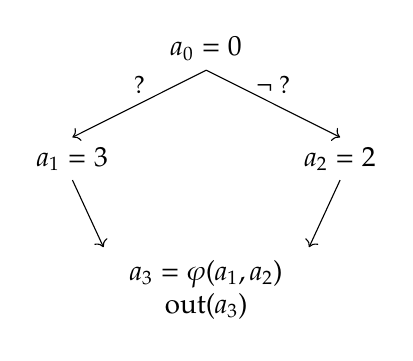
\begin{tikzpicture}[scale=.5]
\node[] (n0) {
  $a_0 = 0$
};
\node[below=of n0] (middle){};
\node[left=of middle] (n1) {
  $a_1 = 3$
};
\node[right=of middle] (n2) {
  $a_2 = 2$
  };
\node[below=of middle] (n3) {
\begin{tabular}{c}
  $a_3 = \phi(a_1, a_2)$ \\
  $\text{out}(a_3)$
\end{tabular}
  };
\draw (n0.south) edge[->] node[above]{\small ?} (n1.north)
      (n0.south) edge[->] node[above]{\small $\neg$ ?} (n2.north)
      (n1.south) edge[->] (n3.north west)
      (n2.south) edge[->] (n3.north east);
\end{tikzpicture}
\end{minipage}

A complete treatment of SSA and many related techniques are available in the excellent [ssabook]. We will still sketch here a few important ideas about SSA, and how they apply more generally.

\paragraph{Dominator tree} A central matter in the SSA transform is the question of where in the program $\phi$ nodes insertions are needed.
This leads us to introduce the notion of domination : we say that a program point $a$ \emph{dominates} another point $b$ if any path in the CFG starting at the root node that reaches $b$ has to go through $a$ first. The domination relation is a partial order over program points and is moreover a tree (every initial segment is well ordered). It is usually called the dominator tree. In our case, since every path to a program point has to go through the head of its containing EBB -- and all the points between the head and itself -- we will say that a program point dominates an EBB if it dominates its head. Given an EBB, the program point being its parent in the dominator tree is called the \emph{immediate dominator}.

The fundamental property of SSA form is then stated as follows : \emph{every use of a variable is dominated by a definition of said variable}. This is, of course, considering $\phi$ nodes as definitions. We can deduce a superset of locations where we have to insert $\phi s$ for the property to hold. We will call the dominance frontier of a program point $a$, noted $DF(a)$, the set of EBB heads that, while not being dominated by $a$, have predecessors that are. $DF(a)$ is the set of nodes that one has to visit in order to, starting from $a$, leave its domination. We note $IDF(a) = \text{lfp}_aDF$. If a variable $v$ has two definitions at $a$ and $b$ respectively, then the set of program points where we have to insert a $\phi$ to disambiguate between $a$ and $b$ are contained in $IDF(a)\cap IDF(b)$. This set is an upper bound, because some of those $\phi$ may end up without any use. Computing the minimal $\phi$ placement is harder and requires a form of liveness analysis. We build the dominator tree and frontiers using the algorithm described in [?].

In its usual formulation, SSA also implies a renaming of every variale to enforce that, as its name indicates, each one has a single definition site. As a consequence, we can store a global $(\text{name}\to\text{value})$ mapping as a flow-insensitive analysis would, but still get flow-sensitive results.

We take a slightly different approach because we compute the SSA form \emph{on the fly} : we assume that use sites of variables cannot be statically determined in advance without computing transfer functions. It also implies that new use and definition sites can be discovered at an already processed program point in later iterations.
The main reason for this choice is to allow for other quantities than variable values to profit from the sparse infrastructure.
[examples]

It is hence inefficient in our case to maintain the renaming property. Instead, when encountering an use, the interpreter walks the dominator tree upward to find the nearest definition. The SSA property guarantees that this lookup can be done following the tree spine, giving it an $O(\text{dominator tree depth})$ worst case complexity. In practice, the dominator tree is very shallow and wide : in the Julia standard library (around 4MB of sources) the deepest dominator tree is of depth [?]. As for the implementation, we do not materialize $\phi$ instructions : they are kept out of band and can be dynamically generated efficiently when required by the discovery of new definitions.

We have not yet witnessed this process to be a bottleneck. Would it become the case, there are several ideas that could be implemented to lower its cost, such as use-forwarding.

% find somewhere to put this
%The choice of EBB for the control flow graph is favorable to forward analysis, as inbound edges are the ones requiring treatment. Even though it is equivalent to a BB graph representation, in practice it allows for a shallower dominator tree.
%Another advantage of EBBs is that the dynamic addition of outbound control flow edges does not require node splitting. It is the case of exception throwing : it would degrade the sparsity of the CFG to conservatively assume that any statement can throw. Our interpreter generates new edges when a transfer function detects a possible raise.

\subsection*{Relational analysis}

[SSA is easy because it handles separable analysis, where the ``diff'' between two states is simply a environment itself. Talk about how the underlying good idea is the summarization between an EBB and it's idom]

\section*{Shape analysis}

\section*{I can see the future}

[technical/impl things] [backward analysis?] [abstract debugger]

We briefly hinted at domain-specific optimizations in the introduction.
Our long term plan is to provide hooks in the compiler and the analyzer to allow for user defined analysis and optimization.
Moreover, those should be able to easily build upon the existing infrastructure.
Although the abstract interpreter model is a good fit in that regard, we have not yet found a fully satisfactory equivalent for the optimization side.

As a good example of the envisioned usefuleness of this kind of modularity, consider the developement of a high-level interface to a BLAS library.
This was not choosen at random since the linear algebra routines are in fact a sizable chunk of the Julia standard library, and BLAS is used as their backend in the common case floating point numeric types.

It is much easier to use under a simple model where the output of the computation is freshly allocated memory containing the result. This avoids aliasing bugs, however it is inefficient because it does not take advantage of the specialized BLAS functions that can output the result in place. Reasonning that the two are equivalent if one of the argument (and all its aliases) are dead after the BLAS call is almost impossible to the compiler because it requires understanding of the routine, of which the core is often hand written assembly. However, the rules of BLAS aliasing are very regular at a high level and someone writing a wrapper for the library could easily, given the right interface, integrate those rules directly as a compiler extension.


\end{document}